\documentclass[12pt,letterpaper]{article}

\usepackage{graphicx}
\usepackage[utf8]{inputenc}
\usepackage{mathtools}
\usepackage[margin=0.5in]{geometry}
\usepackage{booktabs}
\usepackage{tabu}
\usepackage{caption}
\usepackage[labelfont=bf, skip=5pt, font=small]{caption}
\usepackage{hyperref}
\usepackage{siunitx}
\usepackage{standalone}
\usepackage{import}
\usepackage{stanli}


\hypersetup{
    colorlinks=true,
    linkcolor=blue,
    filecolor=magenta,      
    urlcolor=cyan,
    pdftitle={Overleaf Example},
    pdfpagemode=FullScreen,
    }
\usepackage[font=footnotesize,labelfont=bf]{caption}
\setlength{\parskip}{1em}
\setlength{\parindent}{0em}




\let\DeclareUSUnit\DeclareSIUnit
\let\US\SI
\DeclareUSUnit\inch{in}
\DeclareUSUnit\lbf{lbf}
\DeclareUSUnit\lb{lb}
\DeclareUSUnit\psi{psi}
\DeclareUSUnit\ksi{ksi}
\DeclareUSUnit\Msi{Msi}











\begin{document}
\subsubsection{Vehicle Frame}

The vehicle frame has the job of physically constraining each part of the vehicle, and transferring the loads effectively. Bellow is a list of components that need to be constrained and attached to the frame.

\begin{itemize}
\item Motor Mount
\item Flight Computer
\item IMU
\item Battery
\item Landing Legs
\item Vane Assembly
\item Tether Attachment
\end{itemize}

For this scale of vehicle and for the budget. Its important to keep things modifiable, and simple. For this reason I have chosen to use a truss based design. Trusses, especially symmetric trusses are very easy to analyze using hand calculations. However, trusses do add complexity in modeling and can be hard to modify in CAD. This the model method I went with is to define the entire vehicle frame off of one deriving sketch. This 3D sketch will capture the major dimensions of the vehicle, and the location of each joint. Each time a component of the truss is modeled (including clevis attachments and more), it will be deriving from the dimensions of this 3D sketch. This allows major changes to the vehicle, while automatically updating each part in the assembly to meet the new dimensions. 

\begin{figure}[h!]
\centering
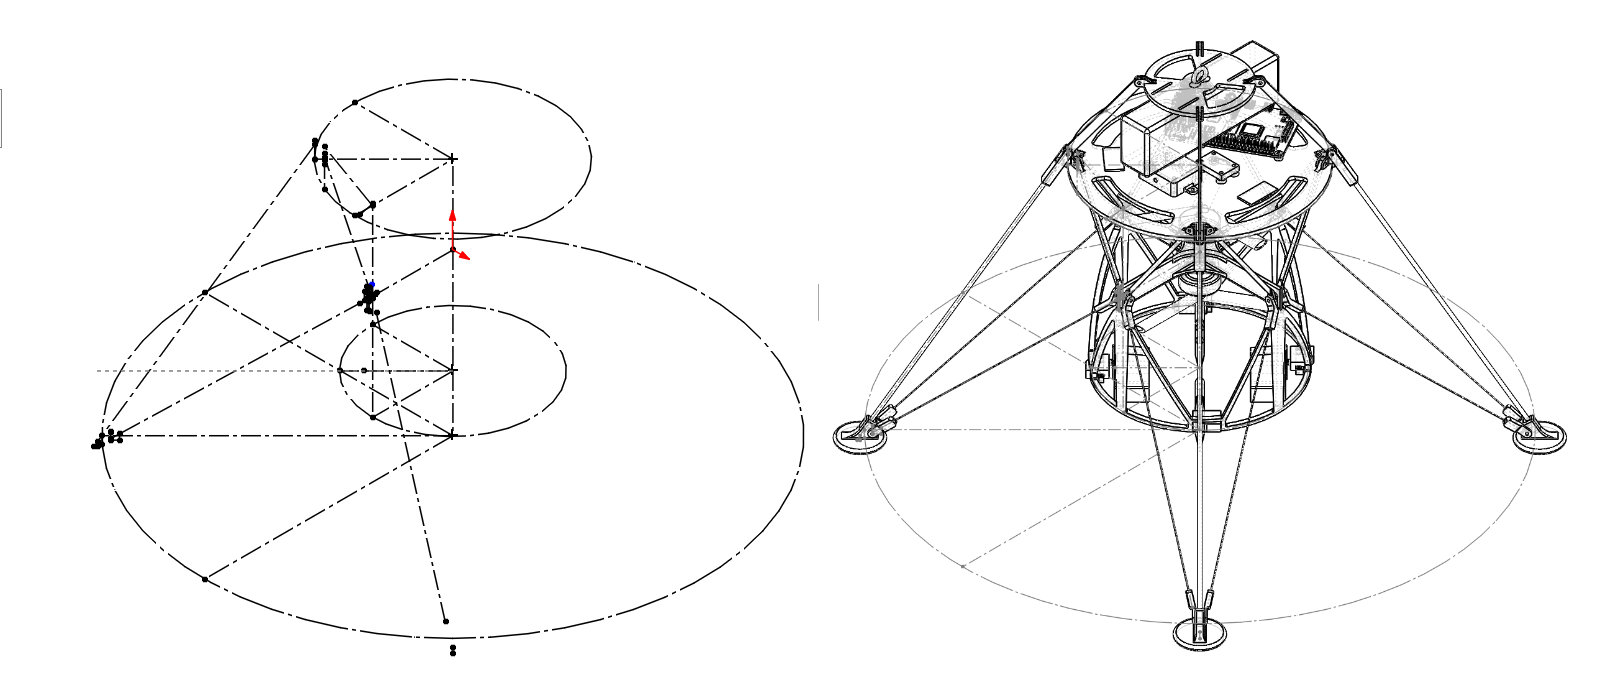
\includegraphics[width = 0.75\textwidth]{Vehicle_Frame_Fig/Deriving_Sketch.png}
\caption*{Deriving Sketch }
\end{figure}

In order to complete the propulsion package and attach it to the vehicle, there needs to be away to fix the control vane assembly to the motor mount. This part will only need to be strong enough to hold the vanes in place, however stiffness needs to be high. If the control vanes bend and flex the fixture, it may lead to inconsistent alignment or unpredictable behavior in flight. Originally I wanted this to be all one piece, however after several attempts to print a cylindrical truss, I will be moving forward with a five piece thrust structure.\\\\

IMAGE of PROP PACKAGE\\\\


The propulsion package needs to be mounted to the avionics and power source. A space truss was constructed to mate the motor mount to the avionics plate.The joints where put as close as possible in attempt to mitigate eccentric loads. During mock assembly, it was noticed that although structural very strong, the weakness in shear of this type of design may be an issue later one.\\\\

IMAGE\\\\

CALCULATIONS ECT\\\\

The last structural member, is the battery and tether mount. For the battery mount, I wanted to keep consistent with many RC aircraft that use battery straps. This allows a variety of battery sizes to be used as well as easy access to swap or charge the current battery. Two standard size RC lipo straps will be used on a mounting plate suspended above the avionics plate. The plate will be supported by four truss members attached to the same joint as the compression strut of the landing gear. \\\\

IMAGE\\\\

CALCS\\\\

Cross section optimization, limited to through hole size!




\end{document}
